% Created by tikzDevice version 0.12.3.1 on 2021-04-08 19:53:14
% !TEX encoding = UTF-8 Unicode
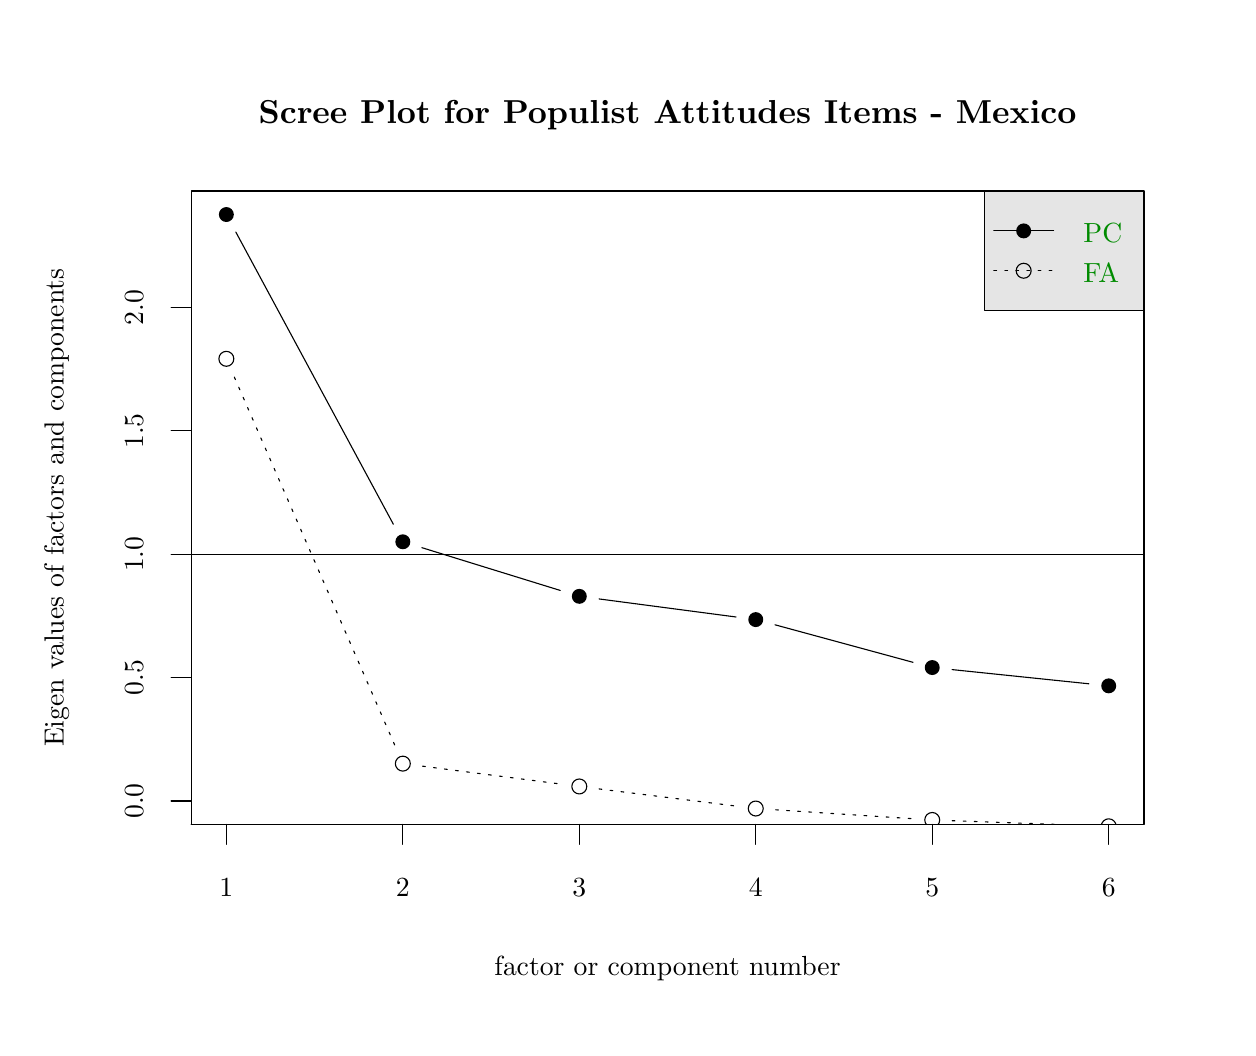
\begin{tikzpicture}[x=1pt,y=1pt]
\definecolor{fillColor}{RGB}{255,255,255}
\path[use as bounding box,fill=fillColor,fill opacity=0.00] (0,0) rectangle (433.62,361.35);
\begin{scope}
\path[clip] ( 59.04, 73.44) rectangle (403.38,302.31);
\definecolor{drawColor}{RGB}{0,0,0}

\path[draw=drawColor,line width= 0.4pt,line join=round,line cap=round] ( 75.21,287.50) -- (132.14,181.91);

\path[draw=drawColor,line width= 0.4pt,line join=round,line cap=round] (142.44,173.45) -- (192.45,157.99);

\path[draw=drawColor,line width= 0.4pt,line join=round,line cap=round] (206.47,154.92) -- (255.95,148.40);

\path[draw=drawColor,line width= 0.4pt,line join=round,line cap=round] (270.04,145.58) -- (319.91,132.02);

\path[draw=drawColor,line width= 0.4pt,line join=round,line cap=round] (334.02,129.39) -- (383.47,124.26);
\definecolor{fillColor}{RGB}{0,0,0}

\path[fill=fillColor] ( 71.79,293.83) circle (  2.70);

\path[fill=fillColor] (135.56,175.57) circle (  2.70);

\path[fill=fillColor] (199.33,155.86) circle (  2.70);

\path[fill=fillColor] (263.09,147.46) circle (  2.70);

\path[fill=fillColor] (326.86,130.13) circle (  2.70);

\path[fill=fillColor] (390.63,123.52) circle (  2.70);
\end{scope}
\begin{scope}
\path[clip] (  0.00,  0.00) rectangle (433.62,361.35);
\definecolor{drawColor}{RGB}{0,0,0}

\path[draw=drawColor,line width= 0.4pt,line join=round,line cap=round] ( 71.79, 73.44) -- (390.63, 73.44);

\path[draw=drawColor,line width= 0.4pt,line join=round,line cap=round] ( 71.79, 73.44) -- ( 71.79, 66.24);

\path[draw=drawColor,line width= 0.4pt,line join=round,line cap=round] (135.56, 73.44) -- (135.56, 66.24);

\path[draw=drawColor,line width= 0.4pt,line join=round,line cap=round] (199.33, 73.44) -- (199.33, 66.24);

\path[draw=drawColor,line width= 0.4pt,line join=round,line cap=round] (263.09, 73.44) -- (263.09, 66.24);

\path[draw=drawColor,line width= 0.4pt,line join=round,line cap=round] (326.86, 73.44) -- (326.86, 66.24);

\path[draw=drawColor,line width= 0.4pt,line join=round,line cap=round] (390.63, 73.44) -- (390.63, 66.24);

\node[text=drawColor,anchor=base,inner sep=0pt, outer sep=0pt, scale=  1.00] at ( 71.79, 47.52) {1};

\node[text=drawColor,anchor=base,inner sep=0pt, outer sep=0pt, scale=  1.00] at (135.56, 47.52) {2};

\node[text=drawColor,anchor=base,inner sep=0pt, outer sep=0pt, scale=  1.00] at (199.33, 47.52) {3};

\node[text=drawColor,anchor=base,inner sep=0pt, outer sep=0pt, scale=  1.00] at (263.09, 47.52) {4};

\node[text=drawColor,anchor=base,inner sep=0pt, outer sep=0pt, scale=  1.00] at (326.86, 47.52) {5};

\node[text=drawColor,anchor=base,inner sep=0pt, outer sep=0pt, scale=  1.00] at (390.63, 47.52) {6};

\path[draw=drawColor,line width= 0.4pt,line join=round,line cap=round] ( 59.04, 81.92) -- ( 59.04,260.21);

\path[draw=drawColor,line width= 0.4pt,line join=round,line cap=round] ( 59.04, 81.92) -- ( 51.84, 81.92);

\path[draw=drawColor,line width= 0.4pt,line join=round,line cap=round] ( 59.04,126.49) -- ( 51.84,126.49);

\path[draw=drawColor,line width= 0.4pt,line join=round,line cap=round] ( 59.04,171.06) -- ( 51.84,171.06);

\path[draw=drawColor,line width= 0.4pt,line join=round,line cap=round] ( 59.04,215.64) -- ( 51.84,215.64);

\path[draw=drawColor,line width= 0.4pt,line join=round,line cap=round] ( 59.04,260.21) -- ( 51.84,260.21);

\node[text=drawColor,rotate= 90.00,anchor=base,inner sep=0pt, outer sep=0pt, scale=  1.00] at ( 41.76, 81.92) {0.0};

\node[text=drawColor,rotate= 90.00,anchor=base,inner sep=0pt, outer sep=0pt, scale=  1.00] at ( 41.76,126.49) {0.5};

\node[text=drawColor,rotate= 90.00,anchor=base,inner sep=0pt, outer sep=0pt, scale=  1.00] at ( 41.76,171.06) {1.0};

\node[text=drawColor,rotate= 90.00,anchor=base,inner sep=0pt, outer sep=0pt, scale=  1.00] at ( 41.76,215.64) {1.5};

\node[text=drawColor,rotate= 90.00,anchor=base,inner sep=0pt, outer sep=0pt, scale=  1.00] at ( 41.76,260.21) {2.0};

\path[draw=drawColor,line width= 0.4pt,line join=round,line cap=round] ( 59.04, 73.44) --
	(403.38, 73.44) --
	(403.38,302.31) --
	( 59.04,302.31) --
	( 59.04, 73.44);
\end{scope}
\begin{scope}
\path[clip] (  0.00,  0.00) rectangle (433.62,361.35);
\definecolor{drawColor}{RGB}{0,0,0}

\node[text=drawColor,anchor=base,inner sep=0pt, outer sep=0pt, scale=  1.20] at (231.21,326.86) {\bfseries Scree Plot for Populist Attitudes Items - Mexico};

\node[text=drawColor,anchor=base,inner sep=0pt, outer sep=0pt, scale=  1.00] at (231.21, 18.72) {factor or component number};

\node[text=drawColor,rotate= 90.00,anchor=base,inner sep=0pt, outer sep=0pt, scale=  1.00] at ( 12.96,187.87) {Eigen values of factors and components};
\end{scope}
\begin{scope}
\path[clip] ( 59.04, 73.44) rectangle (403.38,302.31);
\definecolor{drawColor}{RGB}{0,0,0}

\path[draw=drawColor,line width= 0.4pt,dash pattern=on 1pt off 3pt ,line join=round,line cap=round] ( 74.67,235.09) -- (132.68,102.01);

\path[draw=drawColor,line width= 0.4pt,dash pattern=on 1pt off 3pt ,line join=round,line cap=round] (142.70, 94.49) -- (192.19, 88.09);

\path[draw=drawColor,line width= 0.4pt,dash pattern=on 1pt off 3pt ,line join=round,line cap=round] (206.47, 86.27) -- (255.95, 80.08);

\path[draw=drawColor,line width= 0.4pt,dash pattern=on 1pt off 3pt ,line join=round,line cap=round] (270.28, 78.72) -- (319.68, 75.52);

\path[draw=drawColor,line width= 0.4pt,dash pattern=on 1pt off 3pt ,line join=round,line cap=round] (334.06, 74.79) -- (383.43, 73.03);

\path[draw=drawColor,line width= 0.4pt,line join=round,line cap=round] ( 71.79,241.69) circle (  2.70);

\path[draw=drawColor,line width= 0.4pt,line join=round,line cap=round] (135.56, 95.41) circle (  2.70);

\path[draw=drawColor,line width= 0.4pt,line join=round,line cap=round] (199.33, 87.16) circle (  2.70);

\path[draw=drawColor,line width= 0.4pt,line join=round,line cap=round] (263.09, 79.19) circle (  2.70);

\path[draw=drawColor,line width= 0.4pt,line join=round,line cap=round] (326.86, 75.05) circle (  2.70);

\path[draw=drawColor,line width= 0.4pt,line join=round,line cap=round] (390.63, 72.77) circle (  2.70);

\path[draw=drawColor,line width= 0.4pt,line join=round,line cap=round] ( 59.04,171.06) -- (403.38,171.06);
\definecolor{fillColor}{gray}{0.90}

\path[draw=drawColor,line width= 0.4pt,line join=round,line cap=round,fill=fillColor] (345.86,302.31) rectangle (403.38,259.11);

\path[draw=drawColor,line width= 0.4pt,line join=round,line cap=round] (349.10,287.91) -- (370.70,287.91);

\path[draw=drawColor,line width= 0.4pt,dash pattern=on 1pt off 3pt ,line join=round,line cap=round] (349.10,273.51) -- (370.70,273.51);
\definecolor{fillColor}{RGB}{0,0,0}

\path[fill=fillColor] (359.90,287.91) circle (  2.70);

\path[draw=drawColor,line width= 0.4pt,line join=round,line cap=round] (359.90,273.51) circle (  2.70);
\definecolor{drawColor}{RGB}{0,139,0}

\node[text=drawColor,anchor=base west,inner sep=0pt, outer sep=0pt, scale=  1.00] at (381.50,283.78) {PC };

\node[text=drawColor,anchor=base west,inner sep=0pt, outer sep=0pt, scale=  1.00] at (381.50,269.38) {FA};
\end{scope}
\end{tikzpicture}
